\subsection{RQ1: Difficult topics of new languages}
\label{RQ1}

To answer this research question, we have considered \emph{less answered} questions. By \emph{less answered} question, we imply those questions that have no accepted answer or have an accepted answer but received after the median accepted answer interval of that month. We have calculated the median accepted answer interval for each month of each new language. By accepted answer interval, we imply the time difference between the creation time and time of accepted answer to that question. After accumulating these questions, we have performed LDA  to identify the topics.
 
Difficult topics of Swift are presented below.
\begin{enumerate}
\item \textbf{UI:} UI allows for the interaction between software and its user. UI is the most significant topic for Swift based on Stack Overflow questions. UI questions includes questions like how to achieve this UI function?, how to use multiple UI component like button, audioplayer together? etc.
\topicquote{I have a UIImageView that allows a user ... how to place it in another UIImageView for display when the user pushes that button ...}

\item\textbf{View Controller lifecycle:} View controller is used to manage the app's interface. Questions related to the life cycle of this view controller belong to this category.
\topicquote{I am trying to set up a UIScrollView so that I can swipe between my view controllers ... I just want the whole screen to be a scroll view which allows me to swipe between my view controllers. How would I go about doing that?}

\item \textbf{Mutability:} Immutable variable allows developers to create a variable which will not change ever. It seems developers face problem in the syntax and use of the immutable variable.
\topicquote{I am trying to add an item to my array (which was declared as a var), using anything that might work (+=, append, insert), however, I keep getting the error 'Immutable value of type `AnyObject[]' only has mutating members named `append' ...}

\item \textbf{Data Handling:} It is apparent that Swift developers struggle to interact with video data. This category includes questions which seek for direction like how to save, stream or receive video from network.
\topicquote{I'm playing around with using AVFoundation in Swift Normally when I set up a video camera capture session, I do something like the ... I'm struggling to find how actually to get this working.}

\item \textbf{Migration problem:} Migration problems are two types . (1) The developer is migrating from another language (most of the case Objective-C) and facing problems to mimic the exact logic in Swift, (2) developer is migrating from an old project and facing problem in Xcode. 
\topicquote{I'm not sure if this is something to do with SWIFT or some bug, but I used to be able to call this in objective c ...}
\iffalse
\topicquote{I get this error after adding a Swift class to an old Xcode project. How can I make the project run again?}
\fi

\item \textbf{Documentation clarification:} This category includes questions which seek for the clarification of documentation of Swift itself or its' library.
\topicquote{The documentation I've found is terribly unclear on this - what I'd like to do is use the provided Xcode image library ...}

\iffalse
\textbf{Resource:} This category includes questions which are seeking proper direction and resource. It is apparent that Swift need resources in Swift game development.
\topicquote{I'm trying to replicate the Stanford Matchismo game from "Developing ios apps for iPhone and iPad" in iTunesU in Swift ... Has anyone figured out how to do this yet?  }
\fi
\end{enumerate}

Difficult topics of Go are presented below.
\begin{enumerate}

\item \textbf{Problem in using library:} GRAIL and GORM related problems are the most frequent and is part of this category. Though most of the problems are user specific, it seems they need proper attention.
\topicquote{The following Groovy code creates a GORM-persisted domain class called Foo when written to grails-app ... if I instead write ``public class Foo" the class does NOT get GORM-persisted, I'm running the latest stable release of Grails.}

\item \textbf{Serving request:} This category includes questions which are related to serving request and HTML files in Go language.
\topicquote{What website has some good, up to date resources on using Go HTML/templates, especially in regard to parsing HTML files...}

\item \textbf{Go channel:} Channels are typed conduit through which values can be sent or received. 
\topicquote{I'm very interested in the concurrency model of Google's Go programming language, with very lightweight goroutines and a system of communicating channels...is there an approximation of goroutines or go channels available for C++?}

\item \textbf{Compilation problem:} This category includes questions related to compilation problem. Go language requires a directory structure for compilation. It seems that the structure is not clear to developers.
\topicquote{I noticed the go/ast, go/token, go/parser, etc. packages in the src/pkg/go folder. However, the GCC compiler was based on C files located in src/cmd/gc. My question regards the new go command in Go that builds and runs programs: does this tool depend on the packages I referenced above?...}

\item \textbf{Memory:} Memory allocation and sharing between two separate programs in Go language belong to this category. 
\topicquote{I want to make an array of size N in go, but I don't know what N will be at compile time, how would I allocate memory for it?...}

\item \textbf{Migration problem:} The developers migrating to Go language often seek a solution with reference to the language they migrating from. It means developer expert in another language also faces hard times in Go. 
\topicquote{We want to rewrite kodingen.com backend with Go which currently is Java, running as a daemon using Jsvc. ... I have never touched any C in my life ... simple requirements give me hope that I can start using this wonderful language. What would you advise? Is C still better?}
\end{enumerate}

Difficult topics of Rust are presented below.
\begin{enumerate}

\item \textbf{Use of Struct:} Developers are struggling to get the exact behavior from Rust struct and in destructuring a struct.
\topicquote{I am trying to build a wrapper struct around the ... therefore I need to keep them around. How can I fix this structure? }

\item \textbf{Mutability:} A immutable variable is one which can not change its value after one assignment.
\topicquote{... I ran into trouble when I tried to return a closure that mutates a captured parameter ...}

\item \textbf{Parallel execution:}  Questions related to parallel execution belong to this category.
\topicquote{I am writing a Phoenix client library for Rust, taking advantage of the async WebSocket client from rust-websockets. Right now I am having trouble figuring out how to pass callback functions into the thread that is handling the web socket traffic ... }

\item \textbf{Borrow mechanism:} To access data without taking ownership over it, Rust uses a borrowing mechanism. Developers are facing to determine the scope and when to use it.
\topicquote{I tried to borrow a variable .... it is only saying out of scope }

\item \textbf{Use of Trait:} Rust trait is a collection of methods which can be implemented by any class to use those methods. Developers, especially new developers are facing a hard time to excel in Rust traits.
\topicquote{I'm trying to learn Rust, but I am faced with difficulty when I implement the trait for one of my types.}

\item \textbf{Migration problem:} Like the other two languages, developers migrating to Rust face problems in mimicking logic in Rust.
\topicquote{I am hoping to re-write some parts of a Python project in Rust to speed up things...I am capable of returning complex arrays/structures in Python. And this does not work properly in Rust.}

\iffalse
\item \textbf{Documentation clarification:} Developers often seek clarification about Rust documentation in Stack Overflow. 

\topicquote{I'm an absolute beginner to Rust and systems programming in general. ... I've only come across in C++, but never inline const types. Can someone please provide a beginner-friendly explanation of how this works? )}

\item \textbf{Portability of application:} After developing an application it needs to be delivered to the owners. Developers are facing problem in making portable application with all of their dependencies.

\topicquote{I have a dependency in my Cargo file that needs to be different by platform, specifically, the default features. Here's what I am trying to do ... But this doesn't seem to do what I want. On my Mac it appears to be using the bottom target line as if I just specified hyper = ``0.9". If I do cargo build as specified, I get errors with regard to openssl However, if I build it like this:Then it builds fine. This indicates to me that the cfg for "macos" isn't working while it works for other platform. How do I make this work, or more specifically, how do I solve the dependency which will work for all platforms.)}
\fi
\end{enumerate}

\begin{figure}[htbp]
\centering
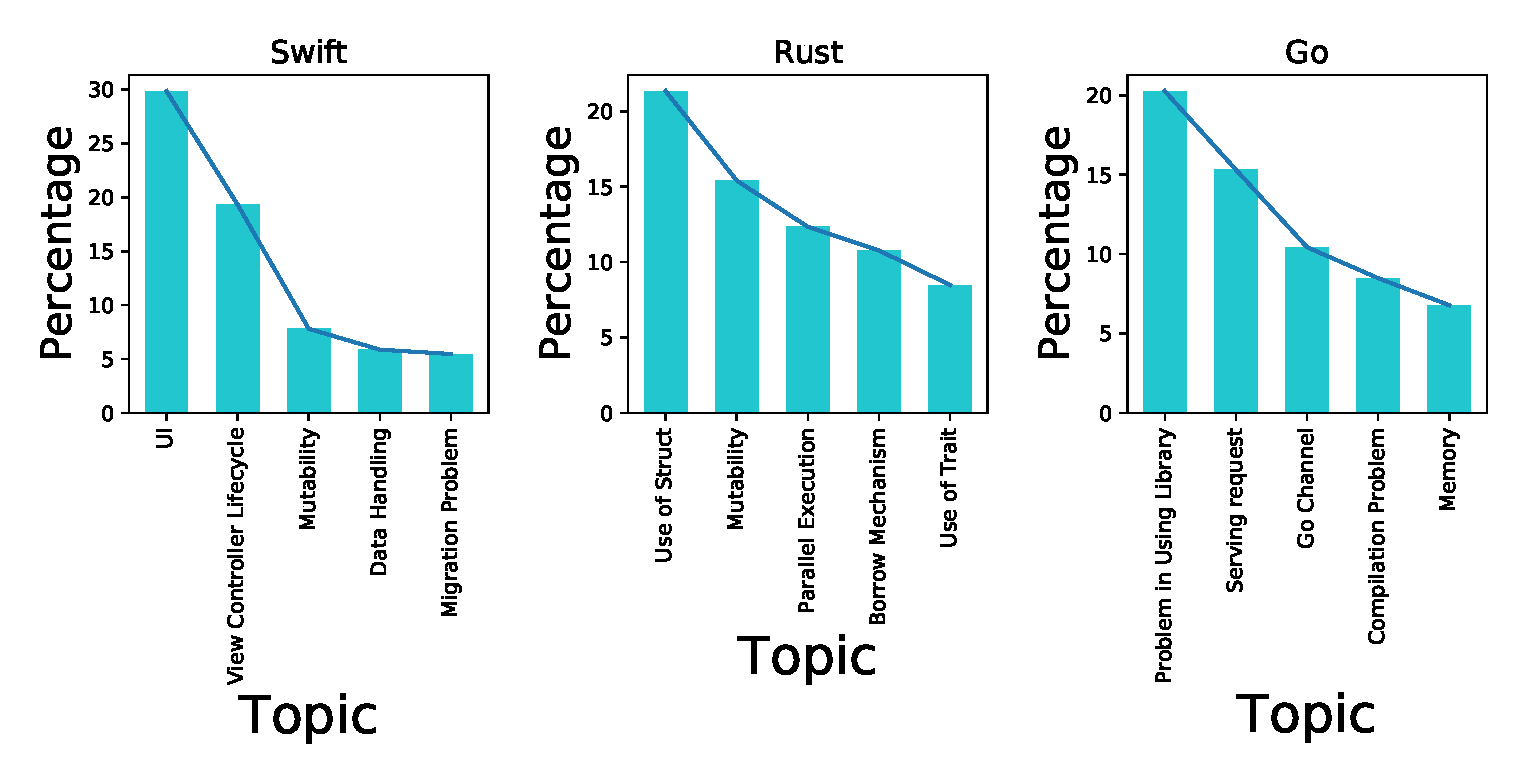
\includegraphics[scale=0.35]{figures/TopicChart.eps}
\caption{Difficult topics of new languages}
\label{fig:less unaswered topics}
\end{figure}

Figure~\ref{fig:less unaswered topics} shows the top 5 difficult topics of new languages with their percentage. It is clear from the topics presented above that the developers of new languages face some problems regardless of the language. 
It is apparent that developers all the three languages face migration problems. 
Another common topic is documentation clarification. Developers ask this type of question as the documentation is not clear or ambiguous. 

\boxtext{\textbf{Finding 1:} In general, questions related to migration and documentation clarification are common in new languages.}